\section{Definitions}
\label{sec:Definitions}

\subsection{Formulation of Agentic Systems}
\label{subsec:Foundation_Model_Based_Agents}


We begin by clarifying the formal definition of an agent. The core of an autonomous agent lies in perceiving its environment, updating its internal state, and performing actions to achieve a specific goal. While such systems have driven decades of AI research, this survey focuses exclusively on a contemporary class: \textit{foundation-model-based agents}, which utilize large foundation models as their central cognitive engines. Crucially, they leverage natural language as a unified interface to integrate perception, reasoning, and tool manipulation. Because a foundation model fundamentally operates as a stateless inference engine, achieving autonomy requires coupling this cognitive core with a persistent, interactive scaffold. Therefore, we formally define the configuration of a foundation-model-based agent at time step $t$ as:
\begin{equation}
\label{eq:agent_formalism}
\mathcal{A}_t \;=\; (\theta_t,\; \Sigma_t),
\end{equation}
where $\theta_t$ encapsulates the neural parameters of the foundation model, and $\Sigma_t$ denotes the agent's dynamic operational scaffold. The scaffold $\Sigma_t$ specifies how the foundation model is conditioned, grounded, and connected to the external world. Concretely, it can be decomposed as
\begin{equation}
\label{eq:scaffold_formalism}
\Sigma_t := (p_t,\, m_t,\, \mathcal{T}_t,\, g_t),
\end{equation}
where $p_t$ denotes structured prompts or system instructions, $m_t$ denotes memory mechanisms and their retrieval and update policies, 
$\mathcal{T}_t$ denotes the set of external tools together with their invocation interfaces, and 
$g_t$ denotes additional control logic such as routing, scheduling, or safety constraints. The interaction between these components and the model's internal parameters is illustrated in Figure \ref{fig:agent_component}, which provides a schematic overview of an FM-based agent within our proposed formalism. Together, 
$\theta_t$ and $\Sigma_t$ determine how the agent reasons, plans, and acts.


During execution, to bridge this intrinsic configuration with the external environment, the agent maintains an ephemeral execution state $X_t$ (e.g., key-value caches, intermediate plans, or short-term working memory) that evolves as it processes an interaction stream. To connect this structural definition to observable behavior, it is beneficial to clarify how the agent's configuration generates its action selection mechanism. Although the foundation model parameters $\theta_t$ implement a general generative distribution, the agent’s realized behavior is jointly determined by both $\theta_t$ and its operational scaffold $\Sigma_t$. Accordingly, we denote the induced policy of the agent based on the foundation model as: 
\begin{equation}\label{policy}
\pi_{\theta_t, \Sigma_t}(A_t \mid X_t),
\end{equation}
where $A_t$ denotes the action produced by the system at time step $t$. Here, the conditioning on $X_t$ captures the transient context of the ongoing interaction. While $X_t$ may strongly influence immediate behavior, it is inherently ephemeral. It is typically discarded or reset once an immediate goal is reached or an external task boundary is crossed, and therefore does not constitute part of the agent's intrinsic architecture. In contrast, the parameters $(\theta_t, \Sigma_t)$ represent the agent's intrinsic configuration over time. While a standard agent may adapt to novel situations by dynamically updating its transient state $X_t$ (e.g., in-context examples), its underlying capabilities remain bounded by its fixed initial setup.

\begin{figure*}[ht]
    \centering
    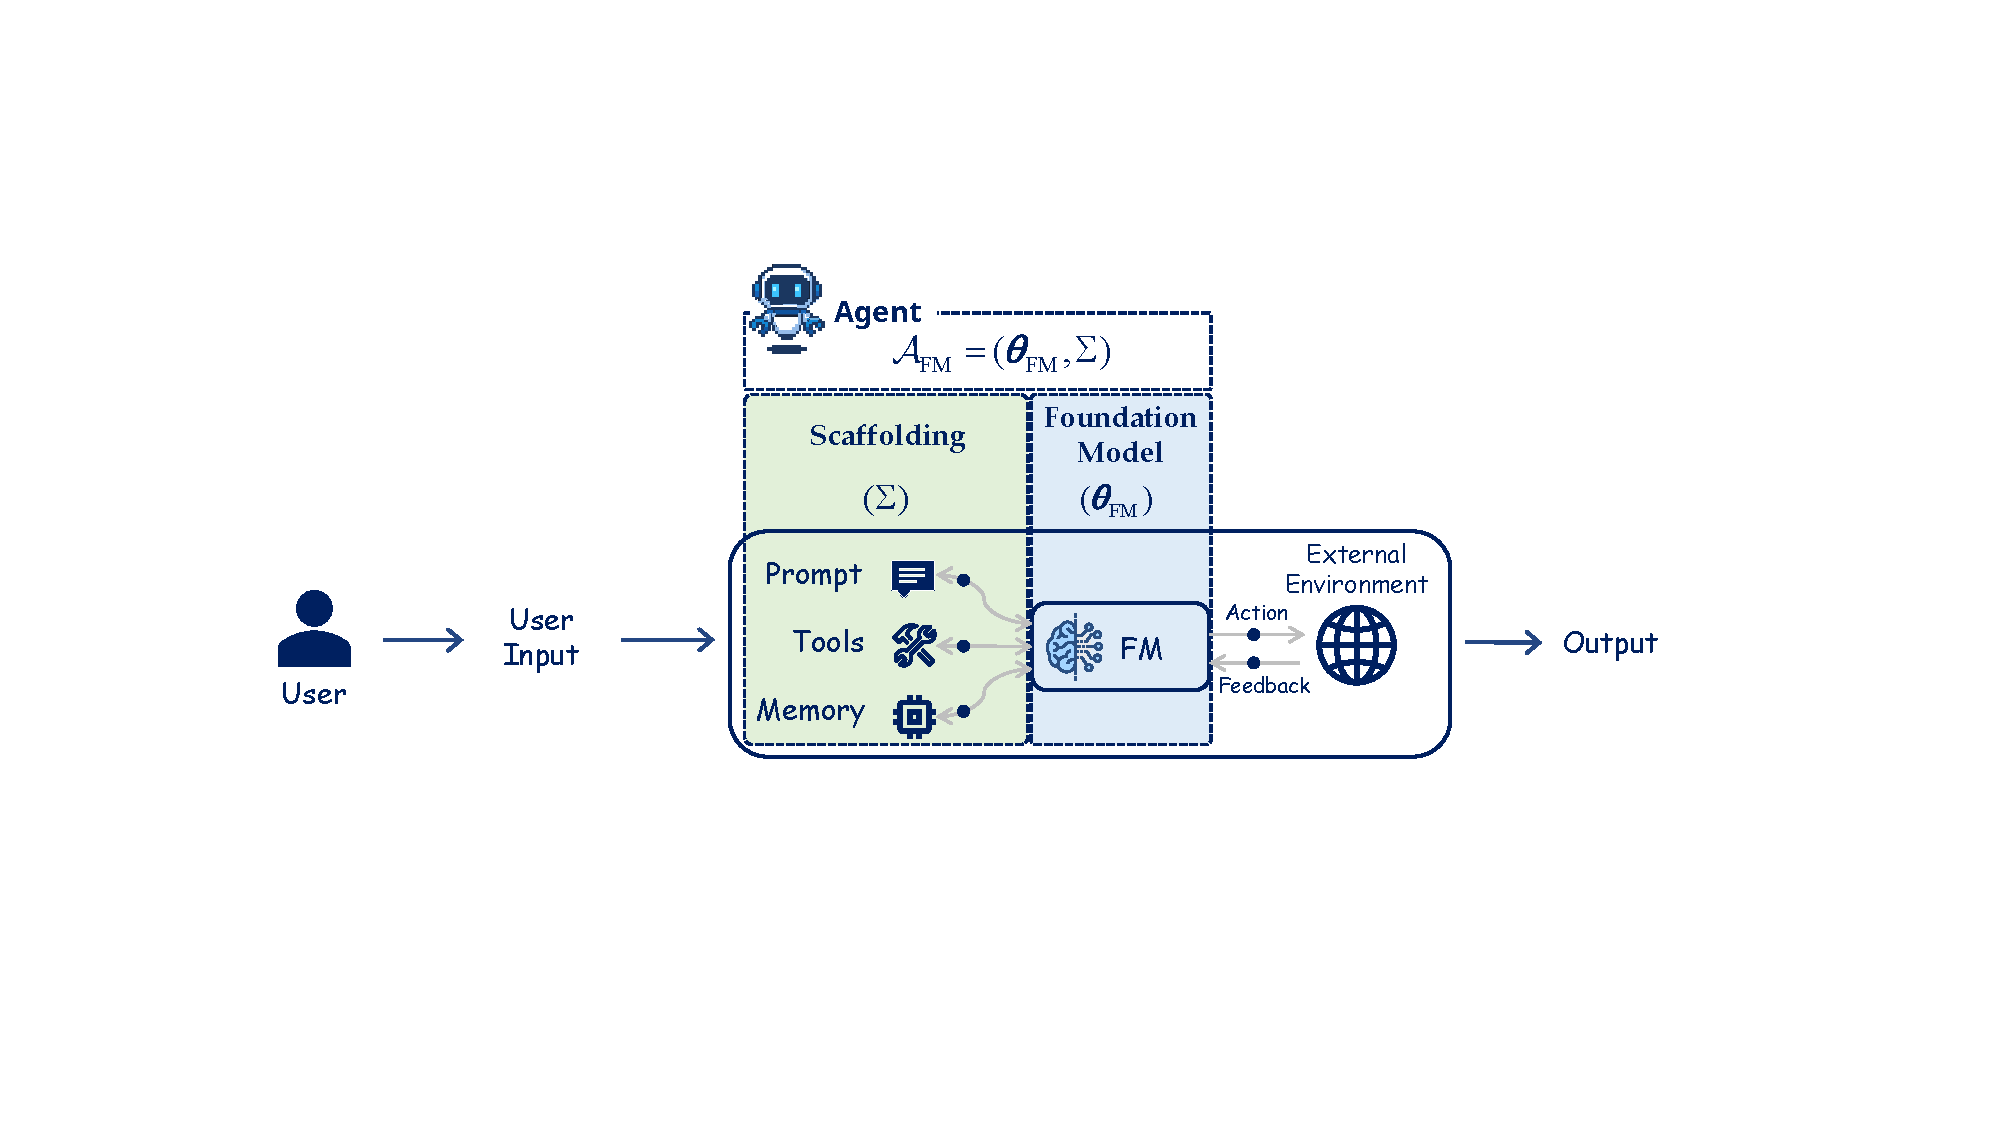
\includegraphics[width=1\linewidth]{fig/agent_component.pdf}
    \caption{Schematic of an FM-based agent under our formalism.}
    \label{fig:agent_component}
\end{figure*}

\subsection{Formal Definition of Self-Improvement}
\label{subsec:Formal_Definition_of_Self_Improvement}


Building upon the formal configuration $\mathcal{A}_t = (\theta_t, \Sigma_t)$, we formalize self-improvement in foundation-model-based agents (SI-FMA) as a process of persistent, endogenous adaptation. Rooted in the foundational principles of explicitly self-referential meta-learning \citep{schmidhuber1987selfreferential, schmidhuber1993self,schmidhuber1997shifting}, a self-improving agent actively leverages signals induced by its own execution---such as interaction outcomes, critiques, verification results, or proposed edits---to durably modify its underlying computational components. 


\paragraph{Self-improvement as a self-induced operator.}
We conceptualize self-improvement through a \emph{self-induced} operator $\mathcal{U}$ that updates the agent’s intrinsic configuration. Let $\pi_{\theta_t,\Sigma_t}$ denote the agent’s induced policy. We formalize this process by factorizing the self-improvement step into an execution phase and an update phase:
\begin{equation}
\mathcal{A}_{t+1} \;=\; \mathcal{U}\Big(\mathcal{A}_{1:t},\; \mathcal{E}\big(\pi_{\theta_{t},\Sigma_{t}};\Sigma_{t},\mathcal{C}_{t}\big)\Big),
\end{equation}
where $\mathcal{E}$ denotes an \emph{agent-executed} procedure that produces a learning signal (e.g., interaction trajectories, reflections, critiques, or proposed edits) by running the induced policy against \textcolor{blue}{a} task context $\mathcal{C}_t$ (e.g., a task distribution, a user interaction stream, or a self-play environment). The scaffold $\Sigma_t$ is included as an explicit argument to $\mathcal{E}$ to permit direct self-inspection (e.g., critiquing prompt templates or auditing tool configurations). 

The system-level update rule $\mathcal{U}$ then applies this self-generated signal to modify the agent's intrinsic components ($\theta$ or $\Sigma$). Unlike the routine evolution of the transient state $X_t$ (e.g., merely accumulating dialogue history or working memory), the operator $\mathcal{U}$ commits durable changes. Crucially, in line with lifelong meta-learning principles, while these updates are not strictly irreversible and may be undone, they allow the agent to consolidate successful strategies into an increasingly stable policy over its interaction stream \citep{Schmidhuber1994OnLH, schmidhuber1995beyond, DBLP:conf/icml/WieringS96, schmidhuber1996simple}.


\paragraph{Two modes of self-reference in SI-FMA.}
SI-FMA may be self-referential in multiple, qualitatively distinct senses. In the first mode, the agent’s policy is executed to \emph{indirectly induce} improvement by generating experience or auxiliary artifacts that serve as learning signals. Self-generated trajectories, evaluations, preferences, or synthetic labels give rise to a learning objective that is subsequently consumed by an update rule, such as an external optimization procedure acting on the foundation model parameters $\theta_t$. This mode realizes self-improvement at the \emph{distributional} level: the agent’s behavior shapes the data and supervision that determine its future parameters.

In the second mode, the agent’s policy is executed to \emph{directly implement} improvements by modifying components of its own operational definition. Through its actions, the agent may edit prompt templates, manage or reorganize memory, reconfigure tool interfaces, or alter control logic, thereby explicitly updating the scaffolding $\Sigma_t$ that governs future execution. In this case, self-improvement is realized through direct, action-level self-modification.

These two modes correspond to distinct but complementary paradigms. \emph{Foundation model improvement} realizes self-improvement through self-induced learning in parameter space, whereas \emph{scaffolding improvement} realizes self-improvement through direct self-modification in execution space. Together, they capture the principal mechanisms by which FM-based agents may alter themselves over time.

\paragraph{Foundation model improvement.}
In foundation model improvement, self-improvement targets the parameters of the underlying foundation model while holding the agent-level scaffolding fixed. Starting from an induced policy $\pi_{\theta_t, \Sigma_t}$, the agent is repeatedly executed in the environment, generating self-induced experience through its own interaction trajectories.

We abstract this process by a self-induced update operator that maps the agent’s current configuration to an updated set of model parameters:
\begin{equation}
\theta_{t+1} = \mathcal{U}_\theta\bigl(\theta_{1:t},\; \mathcal{E}(\pi_{\theta_t, \Sigma_t};\Sigma_t,\mathcal{C}_t)\bigr), \quad \Sigma_{t+1} = \Sigma_t,
\end{equation}
where $\mathcal{C}_t$ is the task or deployment context defined above, $\mathcal{E}$ denotes the execution of the agent under its induced policy in $\mathcal{C}_t$, producing learning signals such as rewards, preference comparisons, synthetic labels, critiques, or verification outcomes, and $\mathcal{U}_\theta$ denotes a parameter-learning procedure that updates the foundation model parameters based on these signals.

Importantly, while the construction of these learning signals may involve rule-based evaluators, learned reward models, or auxiliary model invocations, the underlying data distribution is induced by the agent’s own policy. The operator $\mathcal{U}_\theta$ may instantiate policy-gradient methods, offline or online reinforcement learning, preference optimization, or other parameter-learning algorithms. Foundation model improvement typically operates on longer time scales, incurs substantial computational cost, and leads to stable, global changes in the agent’s internal representations, generalization behavior, and capabilities.

\paragraph{Scaffolding improvement.}
In \emph{scaffolding improvement}, self-improvement targets the agent-level structures surrounding the foundation model while keeping the model parameters $\theta$ fixed. The scaffolding $\Sigma_t$ governs how histories are converted into the conditioning context for the foundation model, how tool calls are specified and executed, how memory is stored and retrieved, and more generally how token sequences are constrained such that they correspond to valid, executable actions. Through these mechanisms, $\Sigma_t$ shapes the agent’s effective observation and action semantics, as well as the construction and evolution of the agent state $X_t$ during execution.

Formally, scaffolding improvement can be expressed as a self-induced update in which an \emph{agent-executed} procedure produces a meta-level signal that is then applied as an intrinsic update:
\begin{equation}
\Sigma_{t+1} \;=\; \mathcal{U}_\Sigma \Big(\Sigma_{1:t},\; \mathcal{E}\big(\pi_{\theta_t,\Sigma_t}; \Sigma_t, \mathcal{C}_t\big)\Big), \qquad \theta_{t+1}=\theta_t,
\end{equation}
where $\mathcal{E}$ denotes the execution of the agent (possibly under a meta-objective) to generate update-relevant artifacts, such as proposed prompt edits, memory reorganizations, tool-interface changes, or new control routines, and $\mathcal{U}_\Sigma$ denotes the system-level mechanism that commits these artifacts as structural scaffolding updates. Unlike the transient evolution of $X_t$, the update above is intended to endure beyond individual task boundaries.

These updates modify the induced policy $\pi_{\theta,\Sigma}$ by reshaping (i) the conditioning context supplied to the foundation model, (ii) the effective action space via admissibility constraints and tool schemas, and (iii) the execution semantics by which token sequences are parsed and grounded into environment actions. Compared to foundation model improvement, scaffolding improvement is typically faster, more reversible, and more context-dependent, yet it can produce substantial changes in the agent’s effective behavior and problem-solving strategies.


\paragraph{Skill as a reusable update.}
The two modes of self-reference above realize self-improvement either indirectly, through self-generated signals that an update rule consolidates into the parameters $\theta$, or directly, through actions that edit the scaffold $\Sigma$; a skill cuts across this distinction. We model a \emph{skill} as a reusable instance of the self-induced update operator $\mathcal{U}$: a named update to the agent's own configuration $\mathcal{A}_t$ that it retains and reuses. Acquiring a skill serializes this update into one of $\mathcal{A}_t$'s substrates: a tool and its calling convention ($\mathcal{T}$), an instruction or workflow ($p$), a memory entry ($m$), consolidated weights ($\theta$), or control logic ($g$). The skill's identity is the update it encodes; the substrate only names where it is stored. This is what makes ``skill'' orthogonal to the substrate axis of our taxonomy. A skill library is then a structured store of, and retrieval policy over, these serialized updates; the same store-and-retrieve structure recurs across substrates, which is why it surfaces in both tool routing and memory organization.

Reusability takes two forms. A skill may be invoked repeatedly, as a retained routine called many times across tasks, or applied once in the manner of an installer: a single update whose value lies in the persistent change it leaves behind, but which remains a portable artifact, reusable across agents and sessions. Either way, a skill is a first-class, serialized operator, in contrast to an ad hoc one-off action that leaves no retained trace.

We further distinguish two scopes according to what an invoked skill acts on. An \emph{object-level} skill acts on the task or world state: invoking it runs a (typically multi-step) routine through the execution operator $\mathcal{E}$ to carry out a sub-task (e.g., a learned \texttt{collect-wood} routine), the agentic analog of a temporally extended option in hierarchical reinforcement learning~\citep{sutton1999between, bacon2017option}. Here the $\mathcal{U}$ step lies in acquisition, which writes the routine into its substrate (e.g., $\mathcal{T}$), not in invocation. A \emph{meta-level} skill instead acts on the agent's own configuration $\mathcal{A}_t$: invoking it edits a component of $\Sigma_t$ or triggers a parameter update (e.g., writing a new tool, refactoring a prompt, consolidating experience into memory, or patching one's own scaffold). The installer-like skills above
are inherently meta-level. For self-improvement, the meta-level scope is the central one. Because a meta-level skill both acts on $\mathcal{A}_t$ and is itself serialized back into $\mathcal{A}_t$, the operator can become part of its own operand. Once such a skill is in turn improved, we recover the self-referential loop in which the improver evolves together with the system it improves~\citep{schmidhuber1987selfreferential, schmidhuber1993self,schmidhuber2003godel}.


Later sections describe how skills are serialized in recent works: as tools (Section~\ref{sec:Tool}), as memory workflows (Section~\ref{sec:Memory}); the application sections illustrate how acquired skills are invoked and reused across tasks.


\subsection{Connections to Related Learning Paradigms}
\label{subsec:Connections_to_Related_Learning_Paradigms}



Because the SI-FMA paradigm is deeply rooted in established learning paradigms, examining it through the lens of these foundational theories offers critical insights. We map SI-FMA onto classical frameworks to clarify where self-improving FM-based agents inherit existing assumptions, where they recombine familiar mechanisms, and where agent architecture makes these mechanisms operationally distinct in practice.

\textbf{Relation to Reinforcement Learning (RL).} 
Classical reinforcement learning provides a natural reference frame for SI-FMA: it formalizes how an agent improves its policy through interaction, and recent work on Agentic RL \citep{zhang2025landscape} extends this view to foundation-model-based agents. Mapping SI-FMA onto this frame clarifies which channels of self-improvement inherit standard RL machinery and which lie outside its formulation. Specifically, updates to $\theta$ correspond to standard policy optimization under a fixed decision process, whereas updates to $\Sigma$ lie outside the standard RL formulation, reshaping the decision process in which the policy operates.

\begin{itemize}
\item \textbf{Parameter updates ($\theta$)}.
When improvement targets the foundation model parameters using interaction trajectories, the process aligns with standard policy optimization. The foundation model acts as a large-scale policy network $\pi_{\theta}$, and techniques such as RLHF \citep{christiano2017deep, ouyang2022training} or self-play optimize $\pi_{\theta}$ via algorithms like Proximal Policy Optimization (PPO) \citep{schulman2017proximal} or Direct Preference Optimization (DPO) \citep{rafailov2023direct}.

\item \textbf{Scaffolding updates ($\Sigma$)}.
When improvement targets the scaffolding, the agent performs a form of structural meta-learning that has no direct counterpart in classical RL. First, whereas classical RL assumes a fixed action space and state representation, updating $\Sigma$ (e.g., adding tools or modifying memory) dynamically alters the effective state-action space and the observation processing logic, thereby reshaping the underlying Markov decision process (MDP) itself. Second, the optimization target itself differs in kind: $\Sigma$ comprises discrete, structured artifacts such as prompts, memory entries, and routing rules, which are typically updated through search, generation, or symbolic edits rather than gradient descent, and which remain explicit and inspectable rather than absorbed into network weights.
\end{itemize}

SI-FMA also departs from classical RL along a second axis: the source of the learning signal. While classical RL relies on external scalar rewards, self-improving agents increasingly utilize self-generated supervision, where the agent acts as its own critic to synthesize feedback signals from its own trajectories, judgments, or verifier modules.


\textbf{Relation to Online Learning.}
Online learning \citep{littlestone1988learning, hoi2021online} studies sequential decision or prediction under a data stream \citep{qi2025webrl}, where the learner updates each round and performance is assessed through cumulative loss or regret. SI-FMA intersects with this view when an agent is updated repeatedly during deployment and evaluation tracks an improvement trajectory rather than a single endpoint, though it is not restricted to the online setting—many self-improvement pipelines operate in batched or offline regimes. Where the paradigms meet, the two channels relate to online learning asymmetrically: $\theta$ updates recover the classical view of updating a hypothesis under a non-stationary stream, whereas $\Sigma$ updates enact a system-level analogue that shifts adaptation to explicit, inspectable components.

\begin{itemize}
    \item \textbf{Parameter updates ($\theta$).}
    These inherit the standard stability challenges of online learning, including distribution shift and catastrophic forgetting. Systems mitigate these risks through controlled update operators such as replay or rehearsal~\citep{robins1995catastrophic}, regularization~\citep{kirkpatrick2017overcoming,ramesh2026learning}, parameter-efficient tuning~\citep{hu2022lora}, and explicit versioning with rollback.

    \item \textbf{Scaffolding updates ($\Sigma$).}
    These provide a channel for rapid adaptation through prompting policies, memory read-write rules, tool routing, and orchestration logic. Externalizing adaptation in this way improves transparency and control, but does not eliminate forgetting and introduces its own failure modes such as memory poisoning, drift in tool semantics, and brittle template dependence.
\end{itemize}


\textbf{Relation to Active Learning.} Active learning studies how a learner selects queries under a labeling budget to maximize information gain, typically by requesting labels from an external oracle \citep{ren2021survey}. SI-FMA intersects with this view when an agent actively controls its data-acquisition process---for example, by targeting frequent failure modes, seeking environments that maximize verifier disagreement, or explicitly requesting human feedback. However, because modern agents often rely on self-generated verification or critiques rather than oracle labels, this behavior transcends standard active learning. It connects SI-FMA directly to classical artificial-curiosity frameworks, in which systems are explicitly designed to actively construct experiments that maximize learning progress, Bayesian surprise, or compression progress~\citep{schmidhuber1991possibility,storck1995reinforcement, schmidhuber2006developmental,schmidhuber2010formal,herrmann2026interestingness}. This perspective places self-improvement within a broader family of curiosity-driven exploration mechanisms, emphasizing that the key design choices are the query policy, the intrinsic objective, and the trustworthiness of the resulting feedback.
